\section{Camera Module}

Camera modules are essential in embedded systems, enabling devices to capture images and videos for processing. These modules consist of an image sensor, lens, and support circuitry, allowing them to connect with microcontrollers and single-board computers. 

They are classified by resolution, power consumption, compatibility, and imaging quality. The OV series from OmniVision, a leading CMOS image sensor supplier, is popular in applications like surveillance, IoT, and computer vision. We will discuss three commonly used models: OV2640, OV7670, and OV5640.

\begin{figure}[h!]
	\centering
	\begin{subfigure}[b]{0.3\textwidth}
		\centering
		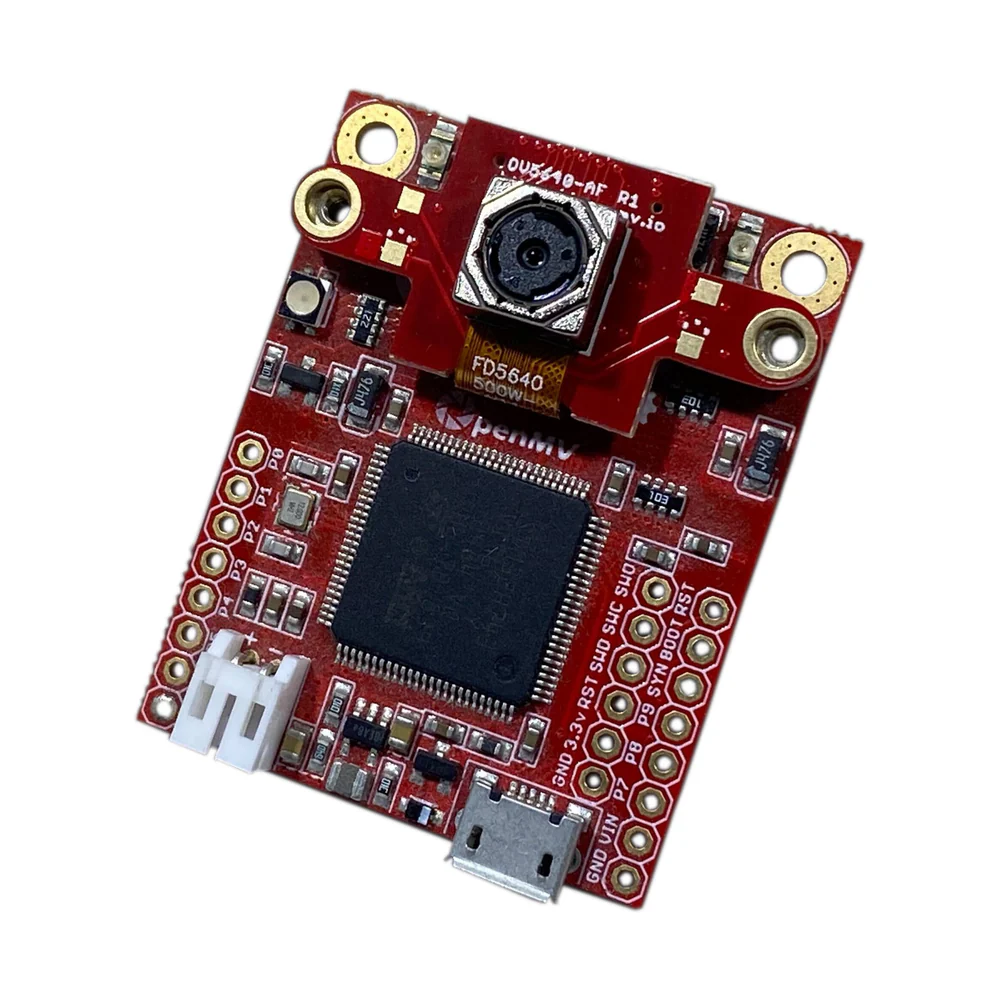
\includegraphics[width=\linewidth]{assets/ch2/OV5640}
		\caption{}
		\label{fig:ov5640}
	\end{subfigure}
	\hfill
	\begin{subfigure}[b]{0.3\textwidth}
		\centering
		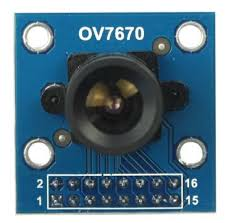
\includegraphics[width=\linewidth]{assets/ch2/OV7670}
		\caption{}
		\label{fig:ov7670}
	\end{subfigure}
	\hfill
	\begin{subfigure}[b]{0.3\textwidth}
		\centering
		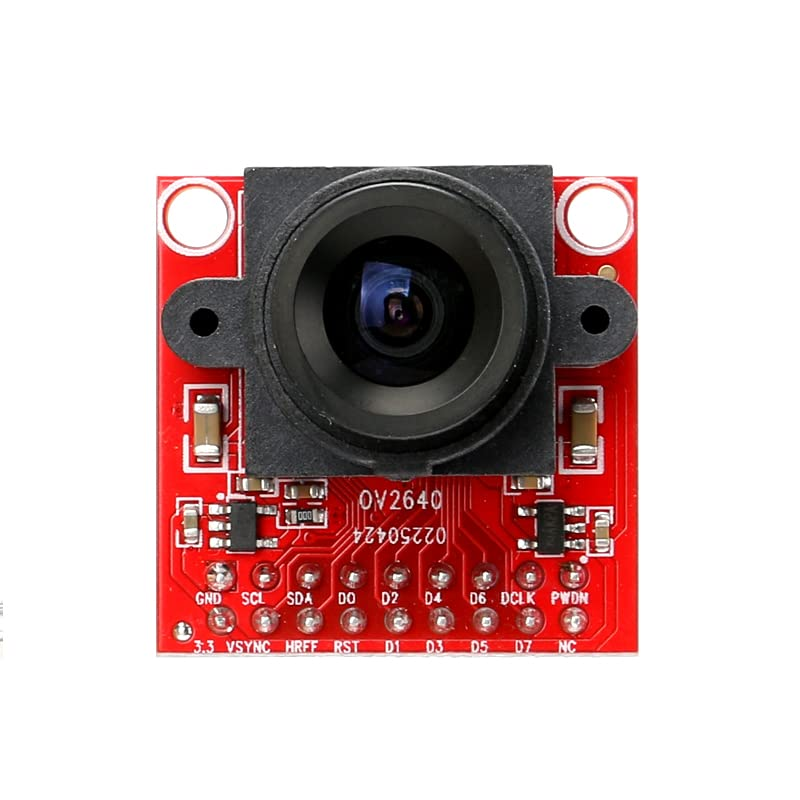
\includegraphics[width=\linewidth]{assets/ch2/OV2640}
		\caption{}
		\label{fig:ov2640}
	\end{subfigure}
	\caption{Camera Modules: (a) OV5640, (b) OV7670, and (c) OV2640}
	\label{fig:camera_modules}
\end{figure}


\begin{itemize}
	\item \textbf{OV2640}: 2MP sensor (1600x1200), outputs in JPEG, YUV, and RGB; low-power module commonly used with ESP32, ideal for IoT due to low-resolution operation and efficient processing. \cite{OV2640}
	
	\item \textbf{OV7670}: 0.3MP VGA sensor (640x480), suitable for basic tasks like color tracking and object detection; low cost and compatible with microcontrollers like Arduino. Includes automatic white balance and gamma correction. \cite{OV7670}
	
	\item \textbf{OV5640}: 5MP sensor (2592x1944), supports JPEG, RAW, and YUV formats; high resolution for applications like facial recognition and barcode scanning, with autofocus and advanced controls. Best for platforms requiring higher processing, like Raspberry Pi. \cite{OV5640}
\end{itemize}







